
Na etapa de pré-processamento, os documentos são pré-processados individualmente conforme são recebidos pelos algoritmos de segmentação extração de tópicos. 
Inicialmente, cada texto passou por um processo de transformação em que as letras foram convertidas em caixa baixa e eliminou-se sinais de pontuação, numerais e termos menores que três caracteres. Em seguida removeu-se os termos que não contribuem para a etapa de segmentação, as quais são chamadas de \textit{stop words}, para identificá-las usou-se uma lista de 438 palavras. Em seguida, extraiu-se o radical de cada palavra por meio da técnica \textit{stemming}. Por fim, selecionou-se os termos com DF \textit{Document Frequency} \leq 2 os quais são considerados mais significativos para tarefas de mineração de texto.



\textit{Stemming}: extraiu-se o radical de cada palavra. Para isso, aplicou-se o algoritmo \textit{Orengo} %\footnote{http://www.inf.ufrgs.br/~viviane/rslp/} para remoção de sufixos~\cite{Alvares2005}.













esses elementos são removidos utilizando uma heurística que varre o texto, detecta a repetição desses elementos e os remove.


Os cabeçalhos são removidos utilizando uma heurística que varre o texto, detecta a repetição desses elementos e os remove.

A eliminação desses termos reduz significativamente o número de termos diminuindo o custo computacional (Manning et al., 2008).






% As atas são normalmente armazenadas em arquivos binários do tipo \textit{pdf}, \textit{doc}, \textit{docx} ou \textit{odt}. As atas devem ser pré-processadas e estruturadas para que possam ser aplicados métodos de MI e RI. Inicialmente, o texto puro é extraído e passa por processos de transformação que incluem o pré-processamento do texto, remoção de elementos considerados menos significativos e a identificação de sentenças. Esse processo é ilustrado na Figura~\ref{fig:preprocessamento-segmentacao} e descrito a seguir.
























% ---------------------------------------------------------------------------------
% ---------------------------------------------------------------------------------

\subsection{Preparação dos documentos}


% ========== Pré-Processamento dos Documentos ==========


\subsection{Pré-Processamento dos Documentos}

As atas são normalmente armazenadas em arquivos binários do tipo \textit{pdf}, \textit{doc}, \textit{docx} ou \textit{odt}. As atas devem ser pré-processadas e estruturadas para que possam ser aplicados métodos de MI e RI. Inicialmente, o texto puro é extraído e passa por processos de transformação que incluem o pré-processamento do texto, remoção de elementos considerados menos significativos e a identificação de sentenças. Esse processo é ilustrado na Figura~\ref{fig:preprocessamento-segmentacao} e descrito a seguir.

	
% -<? Colocar aqui uma explicação do que é um segmento e uma sentença?

\begin{center}
	\begin{figure}[h!]

	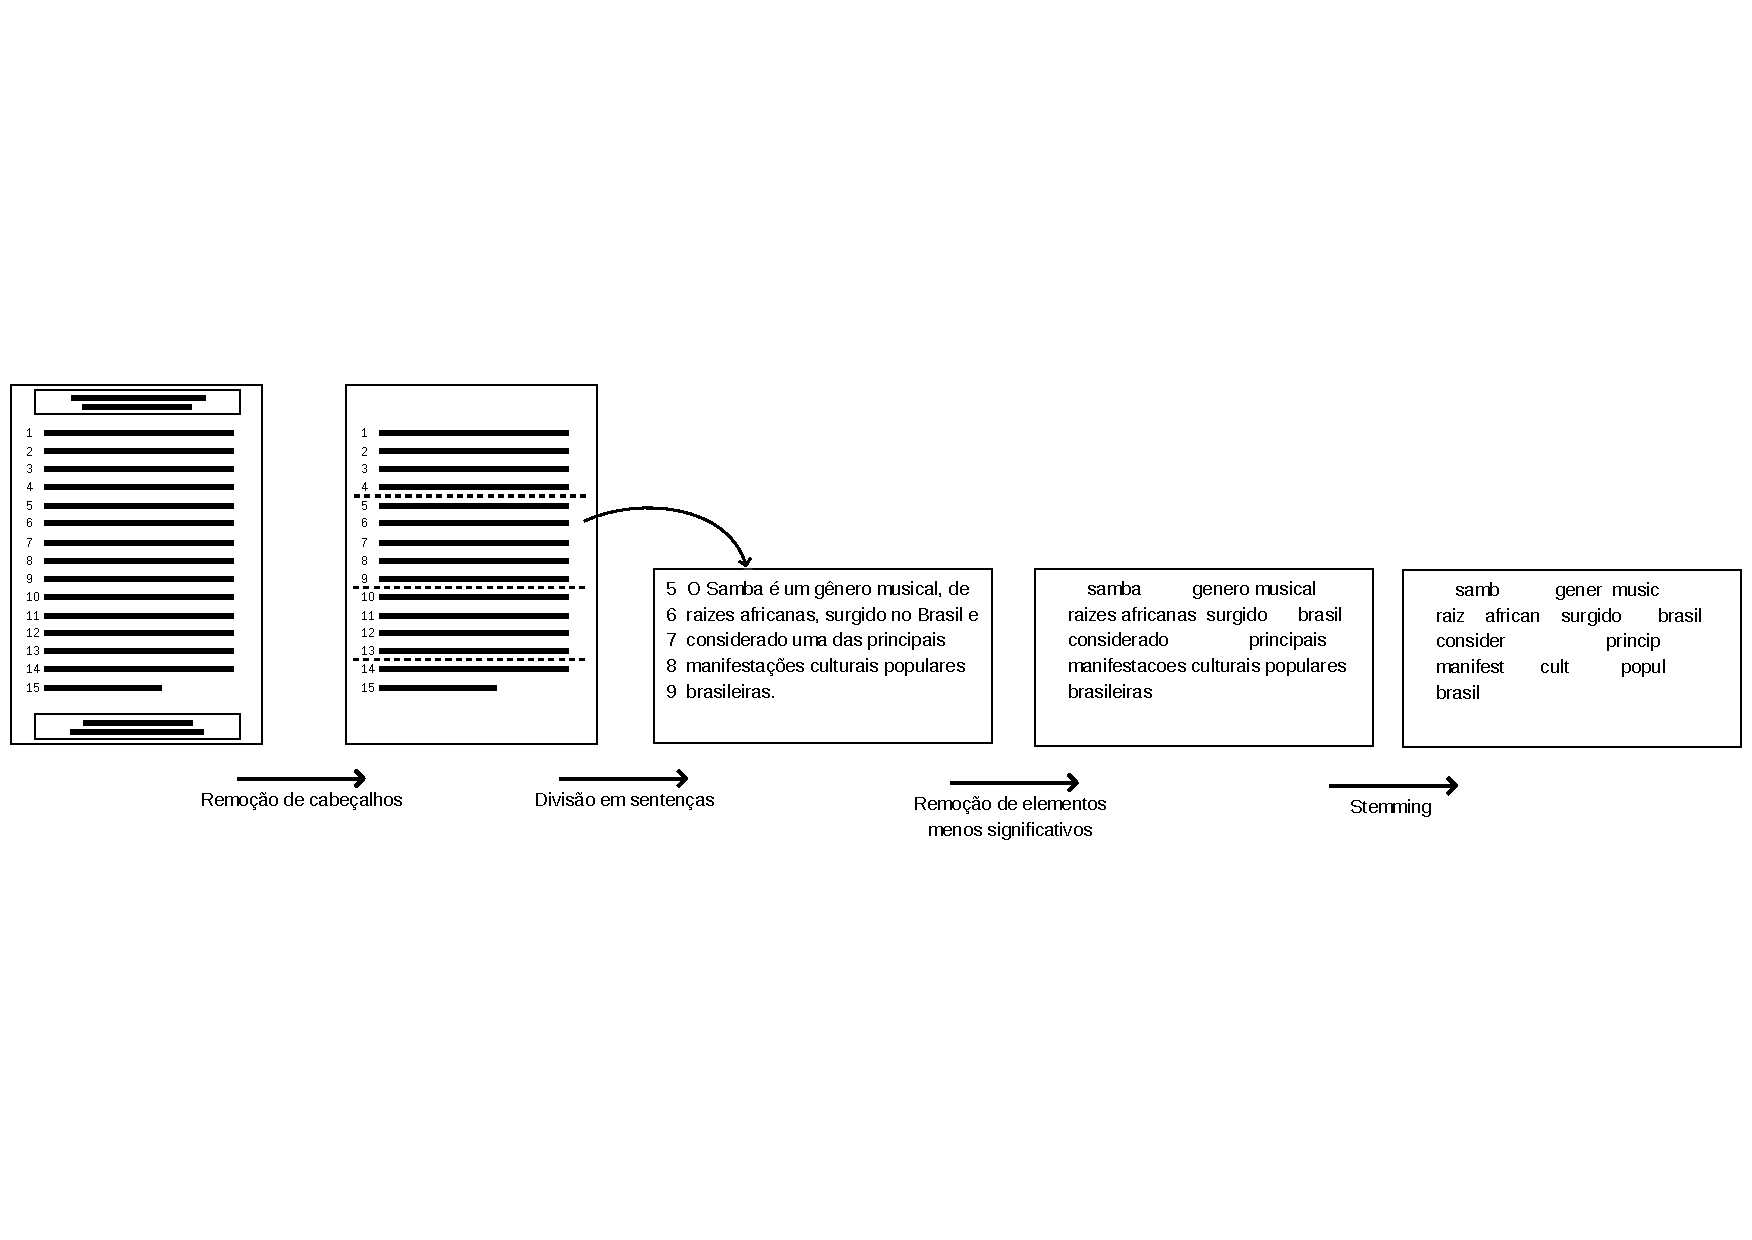
\includegraphics[trim={ 0 180 0 180 },clip,page=1,width=\textwidth]{conteudo/capitulos/figs/pre-process.pdf}

	\caption{Etapa de pré-processamento de um documento que inclui da remoção de elementos menos significativos e a identificação de sentenças}
	\label{fig:preprocessamento-segmentacao}
	\end{figure}
\end{center}



\begin{enumerate}

%  Cabeçalhos e rodapés
\item Remoção de cabeçalhos: as atas contém trechos que podem ser considerados pouco informativos e descartados durante o pré-processamento, como cabeçalhos e rodapés que se misturam aos tópicos tratados na reunião, podendo ser inseridos no meio de um tópico prejudicando tanto os algoritmos de MT e RI, quanto a leitura do texto pelo usuário. Um cabeçalho é a porção de texto que inicia cada página do documento e, de forma semelhante, um rodapé e a porção que as encerra. Detecta-se os cabeçalhos e os rodapés sempre que há uma repetição das primeiras e últimas palavras do documento.


%  Identificação de sentenças
\item Identificação sentenças: Nesse trabalho considera-se as sentenças as menor unidade de informação a ser processada pelos algoritmos de segmentação, por tanto, devem ser identificadas. Ao considerar intuitivamente que uma sentença seja uma sequência de palavras entre sinais de pontuação como ``.'', ``!'' e ``?'', alguns erros poderiam ocorrer quando esses tiverem outra função dentro do texto como em abreviações\footnote{As abreviações são identificadas por meio de uma lista com 234 abreviações conhecidas.}, endereços de internet e datas. Outro problema seriam frases curtas com poucas palavras e que não expressam um conceito completo, mas parte dele. Devido ao estilo de pontuação desses documentos, como encerrar sentenças usando um \textit{``;''} e inserção de linhas extras, foram usadas as regras especiais para identificação de finais de sentença. No Algoritmo~\ref{alg:identificacaofinaisdesent} é mostrado como cada \textit{token} é identificado e marcado com final de sentença.%, esse processo é melhor descrito na Subseção~\ref{subsec:indentificacaosentencas}. % Os detalhes sobre essas regras estão disponíveis para consulta em \urlsoftwares.



\begin{algorithm}
	\SetKwInOut{Input}{Entrada}
	\SetKwInOut{Output}{Saída}
	\SetKwBlock{Inicio}{início}{fim}
	\SetKwFor{ParaTodo}{para todo}{}{fim para todo}
	\SetKwIF{Se}{SenaoSe}{Senao}{}{}{senao se}{senao}{fim se}
	\SetKwFor{Para}{}{}{}
%	\SetKwAlgorithm{Algorithm}{Algoritmo}{}

	
	\Input{Texto}
	\Output{Texto com identificações de finais de sentença}
	
	\ParaTodo {token, marcá-lo como final de sentença se:} {	

	Terminar com um \texttt{!}\\
	Terminar com um \texttt{.} e não for uma abreviação\\
	Terminar em \texttt{.?;} e:
		\Para{}{
			For seguido de uma quebra de parágrafo ou tabulação\\
			O próximo \textit{token} iniciar com  \texttt{(\{["'}\\
			O próximo \textit{token} iniciar com letra maiúscula\\
			O penúltimo caracter  for \texttt{)\}]"'}\\
		}
	}
	
	\caption{Identificação de finais de sentença.}
	\label{alg:identificacaofinaisdesent}
\end{algorithm}


% TODO: "Pra que fazer isso?"


%  Remoção de termos
\item Redução de elementos menos significativos: Removeu-se do textos os termos que não contribuem para a etapa de segmentação, 
	as quais são chamadas de \textit{stop words}. Palavras como artigos, preposições, pronomes, verbos de estado\footnote{Apresentam uma situação inativa, onde o verbo não expressa uma alteração, mas apenas uma propriedade ou condição dos envolvidos.}. Trata-se também como \textit{stop words} as palavras de uso muito frequente dentro de um determinado domínio as quais não são capazes de discriminar textos, portanto também não devem fazer parte dos atributos~\cite{Rezende2003}. Para removê-las, as letras foram convertidas em caixa baixa e usou-se uma lista de 438 palavras para identificá-las. Além disso, eliminou-se a acentuação, sinais de pontuação, numerais e todos os termos menores que três caracteres.

%  Stemming
\item \textit{Stemming}: extraiu-se o radical de cada palavra. Para isso, aplicou-se o algoritmo \textit{Orengo} %\footnote{http://www.inf.ufrgs.br/~viviane/rslp/} 
	para remoção de sufixos~\cite{Alvares2005}.

\end{enumerate}
	


% ---------------------------------------------------------------------------------
% ---------------------------------------------------------------------------------




















































Ao final gerou-se para cada documento uma texto 



"A profª AAA informou que hoje dia cinco de agosto às 14 horas acontecerá a reunião de estruturação do campus e a profª BBB aproveita para esclarecer que essas reuniões tem como objetivo fechar as propostas para que sejam enviadas juntamente com as propostas dos departamentos.",informe,,reunião;estruturação;campus;
"A respeito do PPP do curso da Ciência da Computação a profª AAA informou que o mesmo já está em fase de avaliação na ProGrad e que a comissão que irá avaliá-lo já foi definida.",informe,,ppp;ciência;computação;
"Comunicação dos Membros: O prof. CCC informou que o prof. DDD desistiu de pedir transferência para o nosso campus.",informe,,transferência;desistiu;



\begin{table}[!h]
	\centering 
\footnotesize
	\begin{tabular}{|p{0.2cm}p{14,5cm}|} \hline

		$^{[11]}$&A profª AAA informou que hoje dia cinco de agosto às 14 horas acontecerá a reunião de estruturação do campus e a profª BBB aproveita para esclarecer que essas reuniões tem como objetivo fechar as propostas para que sejam enviadas juntamente com as propostas dos departamentos.
 \\

		$^{[12]}$ &
		A respeito do PPP do curso da Ciência da Computação a profª AAA informou que o mesmo já está em fase de avaliação na ProGrad e que a comissão que irá avaliá-lo já foi definida.\\

		$^{[13]}$ &
		Comunicação dos Membros: O prof. CCC informou que o prof. DDD desistiu de pedir transferência para o nosso campus. 

	\end{tabular}
	\caption{Exemplo de }
	\label{tab:segmentacaoreferencia}
\end{table}










"(II) Encerrada a etapa de inscrição para o processo seletivo como aluno regular para o segundo semestre de 2015: foram quarenta e nove inscrições on-line e dezoito candidatos entregaram a documentação;",informe,,processo;seletivo;

"(III) O Prof. Dr. Alexandre Alvaro informou que a Pró- Reitora comunicou a oferta de mais uma bolsa pela cota da Pró-Reitoria, mas não havia aluno disponível para alocação da bolsa.
O Prof. Dr. José de Oliveira Guimarães informou que havia uma aluna interessada, mas não informada durante o processo de elaboração do ranking no início do semestre.
Ficou decidido enviar e-mail aos docentes solicitando que comuniquem permanentemente interesse de alunos em bolsa pra atualização do ranking;",informe,solicitação;,bolsa;cota;ranking;alunos;
"(IV) Com a mudança do Prof. Dr. Murillo Rodrigo Petrucelli Homem para o campus de São Carlos, o Prof. Dr. José de Oliveira Guimarães assume o posto de suplente da linha Teoria Aplicada à Computação na CPG;",informe,,mudança;suplente;teoria;aplicada;computação;
"Comunicação dos membros: Não houve;",irrelevante,,
"Ordem do Dia: (I) Foram apresentadas regras para participação de membro externo em banca de defesa do mestrado.
O Prof. Dr. Alexandre Alvaro comentou que está sendo pago aos participantes externos das bancas a diária pelo PROAP e o pró-labore pelo DComp, além do programa fornecer o transporte, que onera a verba PROAP.
O Prof. Dr. Tiago Agostinho de Almeida sugeriu o seguinte cálculo para pagamento: se o participante vier de uma Instituição com distância até 220 km será feito o cálculo de R$ 1,00 multiplicado pela quilometragem.
Caso a distância seja superior a 220 km, será calculada a distância multiplicada por R$ 0,60. O menor valor entre o custo do transporte e o pagamento de verba e pró-labore será utilizado para custear a vinda do participante;",informe,discussão;,banca;participantes;diária;transporte;custo;
"(II) Foi discutida a forma de convalidação de disciplinas cursadas como aluno regular anterior a três anos do reingresso do aluno.
Foi decidido que fica a cargo da CPG decidir sobre as disciplinas que serão aproveitadas quando do reingresso do aluno;",decisão,discussão;,disciplinas;aluno;regular;convalidação;

































01 Ata 30 - 26a Reunião Odinária PPGCCS.txt.csv
 7 & 4 & 11 & 6 & 16 & 8 & 8 & 15 & 16 & 
	Anotador  1   7 segmetnos |  25 sentenças
	Anotador  2   4 segmetnos |  25 sentenças
	Anotador  3  11 segmetnos |  25 sentenças
	Anotador  4   6 segmetnos |  25 sentenças
	Anotador  5  16 segmetnos |  25 sentenças
	Anotador  6   8 segmetnos |  25 sentenças
	Anotador  7   8 segmetnos |  25 sentenças
	Anotador  8  15 segmetnos |  25 sentenças
	Anotador  9  16 segmetnos |  25 sentenças
02 Ata 29 - 25a Reunião Odinária PPGCCS.txt.csv
 4 & 4 & 8 & 6 & 11 & 6 & 6 & 15 & 14 & 
	Anotador  1   4 segmetnos |  17 sentenças
	Anotador  2   4 segmetnos |  17 sentenças
	Anotador  3   8 segmetnos |  17 sentenças
	Anotador  4   6 segmetnos |  17 sentenças
	Anotador  5  11 segmetnos |  17 sentenças
	Anotador  6   6 segmetnos |  17 sentenças
	Anotador  7   6 segmetnos |  17 sentenças
	Anotador  8  15 segmetnos |  17 sentenças
	Anotador  9  14 segmetnos |  17 sentenças
03 Ata 36 - 31a Reunião Odinária PPGCCS.txt.csv


 6  & 6  & 8  & 4  & 15 & 9  & 10 & 18 & 14 & 

	Anotador  1   6 segmetnos |  26 sentenças
	Anotador  2   6 segmetnos |  26 sentenças
	Anotador  3   8 segmetnos |  26 sentenças
	Anotador  4   4 segmetnos |  26 sentenças
	Anotador  5  15 segmetnos |  26 sentenças
	Anotador  6   9 segmetnos |  26 sentenças
	Anotador  7  10 segmetnos |  26 sentenças
	Anotador  8  18 segmetnos |  26 sentenças
	Anotador  9  14 segmetnos |  26 sentenças
04 Ata 32 - 28a Reunião Odinária PPGCCS.txt.csv


 5 & 5 & 10 & 6 & 14 & 17 & 7 & 11 & 12 &

	Anotador  1   5 segmetnos |  26 sentenças
	Anotador  2   5 segmetnos |  26 sentenças
	Anotador  3  10 segmetnos |  26 sentenças
	Anotador  4   6 segmetnos |  26 sentenças
	Anotador  5  14 segmetnos |  26 sentenças
	Anotador  6  17 segmetnos |  26 sentenças
	Anotador  7   7 segmetnos |  26 sentenças
	Anotador  8  11 segmetnos |  26 sentenças
	Anotador  9  12 segmetnos |  26 sentenças
05 Ata 33 - 29a Reunião Odinária PPGCCS.txt.csv

 4 & 4 & 6 & 5 & 17 & 22 & 9 & 18 & 16 &

	Anotador  1   4 segmetnos |  33 sentenças
	Anotador  2   4 segmetnos |  33 sentenças
	Anotador  3   6 segmetnos |  33 sentenças
	Anotador  4   5 segmetnos |  33 sentenças
	Anotador  5  17 segmetnos |  33 sentenças
	Anotador  6  22 segmetnos |  33 sentenças
	Anotador  7   9 segmetnos |  33 sentenças
	Anotador  8  18 segmetnos |  33 sentenças
	Anotador  9  16 segmetnos |  33 sentenças
06 Ata 35 - 5a Reunião Extraodinária PPGCCS.txt.csv

3 & 4 & 6 & 4 & 9 & 9 & 4 & 7 & 5 &




	Anotador  1   3 segmetnos |  11 sentenças
	Anotador  2   4 segmetnos |  11 sentenças
	Anotador  3   6 segmetnos |  11 sentenças
	Anotador  4   4 segmetnos |  11 sentenças
	Anotador  5   9 segmetnos |  11 sentenças
	Anotador  6   9 segmetnos |  11 sentenças
	Anotador  7   4 segmetnos |  11 sentenças
	Anotador  8   7 segmetnos |  11 sentenças
	Anotador  9   5 segmetnos |  11 sentenças
07 20ª Reunião Extraordinária CoC-CCS 08-12-10.txt.csv

 3 & 7 & 5 & 4 & 11 & 14 & 5 & 5 & 4 &




	Anotador  1   3 segmetnos |  20 sentenças
	Anotador  2   7 segmetnos |  20 sentenças
	Anotador  3   5 segmetnos |  20 sentenças
	Anotador  4   4 segmetnos |  20 sentenças
	Anotador  5  11 segmetnos |  20 sentenças
	Anotador  6  14 segmetnos |  20 sentenças
	Anotador  7   5 segmetnos |  20 sentenças
	Anotador  8   5 segmetnos |  20 sentenças
	Anotador  9   4 segmetnos |  20 sentenças
08 25ª Reunião Ordinária CoC-CCS 04-04-12.txt.csv

 4 & 8 & 3 & 8 & 12 & 17 & 5 & 11 & 9 &


	Anotador  1   4 segmetnos |  35 sentenças
	Anotador  2   8 segmetnos |  35 sentenças
	Anotador  3   3 segmetnos |  35 sentenças
	Anotador  4   8 segmetnos |  35 sentenças
	Anotador  5  12 segmetnos |  35 sentenças
	Anotador  6  17 segmetnos |  35 sentenças
	Anotador  7   5 segmetnos |  35 sentenças
	Anotador  8  11 segmetnos |  35 sentenças
	Anotador  9   9 segmetnos |  35 sentenças
09 40ª Reunião Ordinária CoC-CCS 06-05-15.txt.csv

3 & 5 & 3 & 6 & 11 & 11 & 3 & 9 & 9 &

	Anotador  1   3 segmetnos |  24 sentenças
	Anotador  2   5 segmetnos |  24 sentenças
	Anotador  3   3 segmetnos |  24 sentenças
	Anotador  4   6 segmetnos |  24 sentenças
	Anotador  5  11 segmetnos |  24 sentenças
	Anotador  6  11 segmetnos |  24 sentenças
	Anotador  7   3 segmetnos |  24 sentenças
	Anotador  8   9 segmetnos |  24 sentenças
	Anotador  9   9 segmetnos |  24 sentenças
10 20ª Reunião Ordinária CoC-CCS 01-06-11.txt.csv

 4 & 5 & 4 & 7 & 31 & 29 & 5 & 9 & 8 &

	Anotador  1   4 segmetnos |  50 sentenças
	Anotador  2   5 segmetnos |  50 sentenças
	Anotador  3   4 segmetnos |  50 sentenças
	Anotador  4   7 segmetnos |  50 sentenças
	Anotador  5  31 segmetnos |  50 sentenças
	Anotador  6  29 segmetnos |  50 sentenças
	Anotador  7   5 segmetnos |  50 sentenças
	Anotador  8   9 segmetnos |  50 sentenças
	Anotador  9   8 segmetnos |  50 sentenças
11 10ª Reunião Ordinária CoC-CCS 05-04-10.txt.csv


4 & 7 & 5 & 7 & 29 & 19 & 5 & 9 & 12 &


	Anotador  1   4 segmetnos |  43 sentenças
	Anotador  2   7 segmetnos |  43 sentenças
	Anotador  3   5 segmetnos |  43 sentenças
	Anotador  4   7 segmetnos |  43 sentenças
	Anotador  5  29 segmetnos |  43 sentenças
	Anotador  6  19 segmetnos |  43 sentenças
	Anotador  7   5 segmetnos |  43 sentenças
	Anotador  8   9 segmetnos |  43 sentenças
	Anotador  9  12 segmetnos |  43 sentenças
12 13ª Reunião Ordinária CoC-CCS 05-08-10.txt.csv

3 & 10 & 4 & 16 & 33 & 25 & 4 & 13 & 11 &


	Anotador  1   3 segmetnos |  56 sentenças
	Anotador  2  10 segmetnos |  56 sentenças
	Anotador  3   4 segmetnos |  56 sentenças
	Anotador  4  16 segmetnos |  56 sentenças
	Anotador  5  33 segmetnos |  56 sentenças
	Anotador  6  25 segmetnos |  56 sentenças
	Anotador  7   4 segmetnos |  56 sentenças
	Anotador  8  13 segmetnos |  56 sentenças
	Anotador  9  11 segmetnos |  56 sentenças




% Entre os principais trabalhos da literatura podemos citar o \textit{TextTiling} ~\cite{Hearst1994} e o \textit{C99}~\cite{Choi2000} são considerados um dos primeiros mais influentes sendo utilizados com \textiit{base lines} em trabalhos recentes~\cite{CHAIBI2014, Naili2016, Cardoso2017}


% para então ser segmentação do texto em trechos com um assunto predominante. 
% conforme apresentados a seguir.

% melhorar ↓↓↓↓↓
% A seguir são apresentadas as etapas do módulo de preparação e manutenção desde a preparação dos documentos até a entrega da estrutura interna ao módulo de consulta. 





% A Figura~\ref{fig:preprocessamento-segmentacao} mostra a etapa de preparação de um documento em português que inclui a remoção de elementos menos significativos e a identificação de sentenças e segmentos.


  % A Figura \ref{fig:visao-geral} mostra a visão geral do sistema com suas principais entradas e saídas. 



e devolve o histórico de menções 


informações extraídas


0. Extração e preparação do texto

1. Segmentação dos documentos

2. Extração dos tópicos


















% --> Encerramento da seção de segmentação.
Ao final do processo de segmentação, são produzidos fragmentos de documentos, aqui chamados de subdocumentos. Esses subdocumentos contém um texto, assim como no documento original, em um estágio de processamento inicial, pois ainda não estão estruturados. Ocorre que as técnicas de aprendizado de máquina exigem uma representação estruturada dos textos conforme será visto na Seção~\ref{section:RepTextos}.




% Analisou-se também o desempenho da mesma técnica aplicada a um texto contínuo extraído de artigo da Internet que descreve seis gêneros musicais brasileiros um após um outro separados em seções. Ao observar a Figura~\ref{fig:coesaolexicaTT-generos-musicais}, nota-se que os vales são mais definidos e a maioria dos segmentos coincidem ou estão próximos a segmentação de referência. A segmentação de referência possui sete segmentos que separam uma introdução do assuntos e respeitam cada uma das subseções que tratam de um gênero musical. Obtém-se nesse cenário uma eficiência maior em relação a segmentação da ata, o que sugere que textos organizados em seções podem ter melhores benefícios com técnicas baseadas em coesão léxica que as atas, onde esse fator é menos significativo.  % ou a premissa do algoritmo não é tão boa.



  % %--- ---
  % \begin{figure}[!h]
	  % \centering
	  % 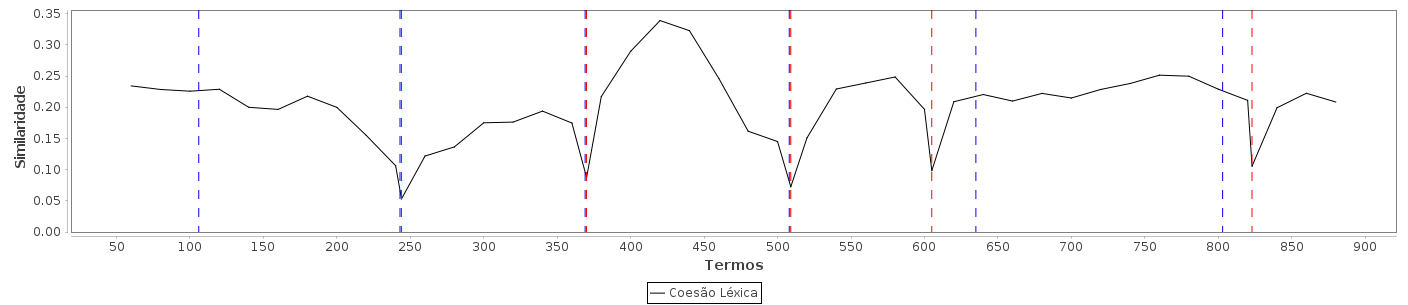
\includegraphics[width=\textwidth]{conteudo/capitulos/figs/generos-musicais-TT-40-20.png}
	  % \caption{Variação da coesão léxica ao longo de um artigo melhor estruturado em seções junto a uma segmentação automática em contraste com uma segmentação de referência.}
	  % \label{fig:coesaolexicaTT-generos-musicais}
  % \end{figure}
